%%%%%%%%%%%%%%%%%%%%%%%%%%%%%%%%%%%%%%%%%%%%%%%%%%%%%%%%%%%%%%%%%%%
% 
% $Id: ap1.tex,v 1.1.1.1 2002/01/02 19:36:48 phil Exp $
%
% $Log: ap1.tex,v $
% Revision 1.1.1.1  2002/01/02 19:36:48  phil
% initial import into CVS
%
% Revision 1.3  1997/08/28 16:40:01  cguo
% *** empty log message ***
%
% Revision 1.2  1996/04/29 19:05:38  stockie
% ready for carmen
%
% Revision 1.1  1995/08/29  21:06:41  stockie
% Initial revision
%
% Revision 1.2  1995/06/29  21:26:21  stockie
% *** empty log message ***
%
%
%%%%%%%%%%%%%%%%%%%%%%%%%%%%%%%%%%%%%%%%%%%%%%%%%%%%%%%%%%%%%%%%%%%

\section{Mathematical Notes}
\label{lab2:ap:mathnote}

%%%%%%%%%%%%%%%%%%%%%%%%%%%%%%%%%%%%%%%%%%%%%%%%%%%%%%%%%%%%%%%%%%%%%
\subsection{Taylor Polynomials and Taylor Series}
\label{lab2:ap:taylor-series}

Taylor Series are of fundamental importance in numerical analysis.
They are the most basic tool for talking about the approximation of
functions.
Consider a function $f(x)$ that is smooth -- when we say ``smooth'',
what we mean is that its derivatives exist and are bounded (for the
following discussion, we need $f$ to have $(n+1)$
derivatives).  
We would like to approximate $f(x)$ near the point $x=x_0$, and we
can do it as follows:
\[
  f(x) = \underbrace{P_n(x)}_{\mbox{\rm Taylor polynomial}} +
  \underbrace{R_n(x)}_{\mbox{\rm remainder term}},
\]
where 
\[
  P_n(x)=f(x_0)+ f^\prime(x_0)(x-x_0) +
  \frac{f^{\prime\prime}(x_0)}{2!}(x-x_0)^2 + \cdots + 
  \frac{f^{(n)}(x_0)}{n!}(x-x_0)^n 
\]
is the \emph{ $n$th order Taylor polynomial} of $f$ about $x_0$, and
\[
  R_n(x)=\frac{f^{(n+1)}(\xi(x))}{(n+1)!}(x-x_0)^{n+1}
\]
is the \emph{ remainder term} or \emph{ truncation error}.
The point $\xi(x)$ in the error term lies somewhere between the points
$x_0$ and $x$.
If we look at the infinite sum (\ie~let $n\rightarrow\infty$), then
the resulting infinite sum is called the \emph{ Taylor series of $f(x)$ about
  $x=x_0$}.  
This result is also know as \emph{ Taylor's Theorem}.

Remember that we assumed that $f(x)$ is smooth (in particular, that
its derivatives up to order $(n+1)$ exist and are finite).
That means that all of the derivatives appearing in $P_n$ and $R_n$
are bounded.
Therefore, there are two ways in which we can think of the Taylor
polynomial $P_n(x)$ as an 
approximation of $f(x)$:
\begin{enumerate}
\item First of all, let us fix $n$.  
  Then, we can improve the approximation by letting $x$ approach
  $x_0$, since as $(x-x_0)$ gets small, the error term $R_n(x)$ goes
  to zero ($n$ is considered fixed and all terms depending on $n$ are
  thus constant).  Therefore, the approximation improves when $x$ gets
  closer and closer to $x_0$.
\item Alternatively, we can think of fixing $x$.  Then, we can improve
  the approximation by taking more and more terms in the series.  When
  $n$ is increased, the factorial in the denominator of the error term
  will eventually dominate the $(x-x_0)^{n+1}$ term (regardless of how
  big $(x-x_0)$ is), and thus
  drive the error to zero.
\end{enumerate}
In summary, we have two ways of improving the Taylor polynomial
approximation to a function: by evaluating it at points closer to the
point $x_0$; and by taking more terms in the series.

\begin{example}
  This property of the Taylor expansion can be seen by a simple example.
  Consider the Taylor polynomial for the function
  $f(x)=\sin(x)$ about the point $x_0=0$.  All of the even terms are
  zero, so that if we take $n$ odd (\ie~$n=2k+1$), then the $n$th
  order Taylor polynomial is
  \[
    P_{2k+1}(x)=x+\frac{x^3}{3!}+\frac{x^5}{5!}+\frac{x^7}{7!}+\cdots
    +\frac{x^{2k+1}}{(2k+1)!}. 
    \]

  The plot in Figure~\ref{lab2:fig:taylor-series} illustrates quite clearly
  how the approximation improves both as $x$ approaches 0, and as $n$ is
  increased.  
  \begin{figure}[htbp]
    \begin{center}
      \leavevmode
      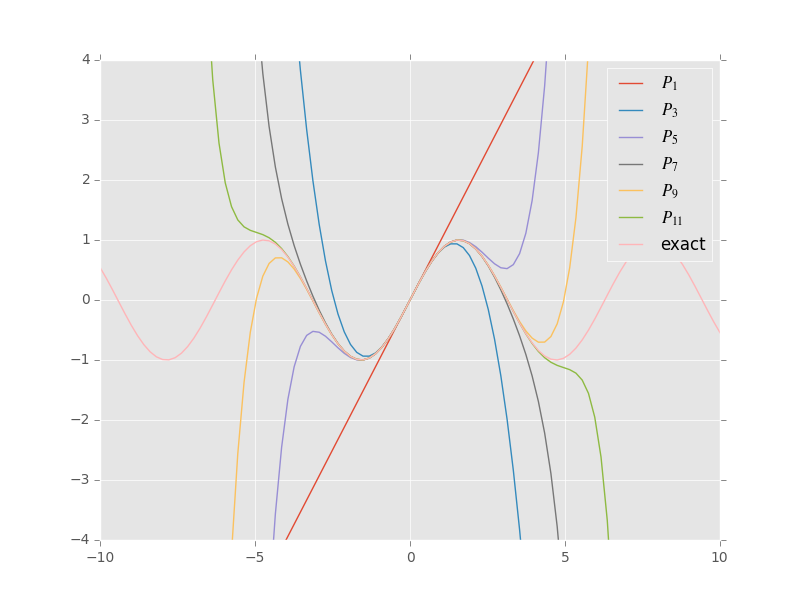
\includegraphics[height=3.5in]{taylor/taylor}
    \end{center} 
    \caption{Plot of $\sin(x)$ compared to its Taylor polynomial
      approximations about $x_0=0$, for various values of $n$.}
    \label{lab2:fig:taylor-series}
 \end{figure}
  Consider a specific Taylor polynomial, say $P_3(x)$ (\ie~fix $n=3$).
  Notice that for $x$ far away from the origin, the polynomial is
  nowhere near the function $\sin(x)$.  However, it approximates the
  function quite well near the origin.
  On the other hand, we could take a specific point, $x=5$, and notice
  that the Taylor series of orders 1 through 7 do not approximate the
  function very well at all.  
  Nevertheless the approximation improves as $n$ increases, as is shown
  by the 15th order Taylor polynomial.
\end{example}

%%%%%%%%%%%%%%%%%%%%%%%%%%%%%%%%%%%%%%%%%%%%%%%%%%%%%%%%%%%%%%%%%%%%%
\subsection{Floating Point Representation of Numbers}
\label{lab2:ap:floating-point}

Unlike a mathematician, who can deal with real numbers having infinite
precision, a computer can represent numbers with only
a finite number of digits.  
The best way to understand how a computer stores a number is to look at
its \emph{ floating-point form}, in which a number is written as
\[
\pm 0.d_1 d_2 d_3 \ldots d_k \times 10^n,
\]
where each digit, $d_i$ is between 0 and 9 (except $d_1$, which must
be non-zero).  
Floating point form is commonly used in the physical sciences to
represent numerical values; for example, the Earth's radius is
approximately 6,400,000 metres, which is more conveniently written in
floating point form as $0.64\times 10^7$ (compare this to the general
form above).

\begin{note}
  Computers actually store numbers in \emph{ binary form} (i.e.\ in
  base-2 floating point form, as compared to the decimal or base-10 
  form shown above).  However, it is more convenient to use the
  decimal form in order to illustrate the basic idea of computer
  arithmetic.  For a good discussion of the binary representation of
  numbers, see Burden \& Faires ~\cite[sec.~1.2]{burden-faires}.  
\end{note}

For the remainder of this discussion, assume that we're dealing with a
computer that can store numbers with up to 8 \emph{ significant digits}
(i.e.~$k=8$) and exponents in the range $-38 \leq n \leq 38$.
Based on these values, we can make a few observations regarding the
numbers that can be represented:
\begin{itemize}
\item The largest number that can be represented is about $1.0\times
  10^{+38}$, while the smallest is $1.0\times 10^-38$.  
\item These numbers have a lot of \emph{ holes}, where real numbers are
  missed.  For example, consider the two consecutive floating point
  numbers 
  \[
  0.13391482 \times 10^5 \;\;\; {\rm and} \;\;\; 0.13391483 \times 10^5,
  \]
  or 13391.482 and 13391.483.  Our floating-point number system cannot
  represent any numbers between these two values, and hence any number
  in between 13391.482 and 13391.483 must be approximated by one of the
  two values.  Another way of thinking of this is to observe that 
  $0.13391482 \times 10^5$ does not represent just a single real number,
  but a whole \emph{ range} of numbers. 
\item Notice that the same amount of floating-point numbers can be
  represented between $10^{-6}$ and $10^{-5}$ as are between $10^{20}$
  and $10^{21}$.  Consequently, the density of floating points numbers
  increases as their magnitude becomes smaller.  That is, there are
  more floating-point numbers close to zero than there are far away.
  This is illustrated in the Figure~\ref{lab2:fig:float}.
  \begin{figure}[htbp]
    \begin{center}
      \leavevmode
      \htmlimage{scale=1.5}
      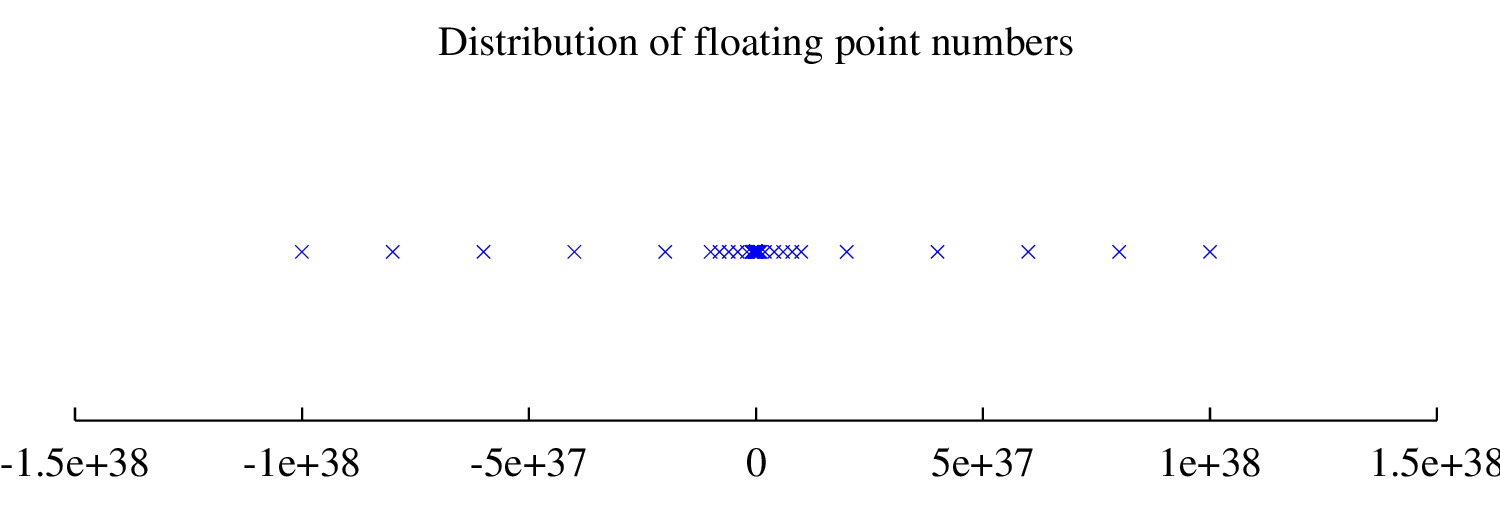
\includegraphics[width=5.0in]{float/float1}
      \caption{The floating-point numbers (each represented by a
        $\times$) are more dense near the origin.} 
      \label{lab2:fig:float}
    \end{center}
  \end{figure}
\end{itemize}
 
The values $k=8$ and $-38\leq n \leq 38$ correspond to what is known
as \emph{ single precision arithmetic}, in which 4 bytes (or units of
memory in a computer) are used to store each number.  It is typical in
many programming languages, including $C++$, to allow the use of higher
precision, or \emph{ double precision}, using 8 bytes for each number,
corresponding to values of $k=16$ and $-308\leq n \leq 308$, thereby
greatly increasing the range and density of numbers that can be 
represented.  When doing numerical computations, it is customary to
use double-precision arithmetic, in order to minimize the effects of
round-off error (in a $C++$ program, you can define a
variable \texttt{ x} to be double precision using the declaration \texttt{
  double x;}). 

\begin{note}
  Sometimes, double precision arithmetic may help in eliminating
  round-off error problems in a computation.  
  On the minus side, double precision numbers require more storage
  than their single precision counterparts, and it is sometimes
  (but not always) more costly to compute in double precision.
  Ultimately, though, using double precision should not be expected to
  be a cure-all against the difficulties of round-off errors.
  The best approach is to use an algorithm that is not unstable with
  respect to round-off error.  For an example where increasing
  precision will not help, see the section on
  Gaussian elimination in
  Lab~\#3.\externalref{lab3:sec:round-off-error}  
\end{note}

%%% Local Variables: 
%%% mode: latex
%%% TeX-master: "lab2"
%%% End: 
